%!TEX root = ../master_thesis.tex
\chapter{Background}
\label{ch:background}
In this thesis, we work with methods from signal processing and machine learning. In this chapter, we first start with a brief introduction to audio signal processing in Section~\ref{sec:asp} and build the foundation for the later part of the thesis. Later we follow our discussion and build concepts of deep learning with a particular focus on deep generative models in Section~\ref{sec:dgm}.

\section{Audio Signal Processing}
\label{sec:asp}
Audio signal processing (ASP) deals with the perception of sound to human auditory system. The physical form of sound or an audio signal can be seen as an encoding of air pressure over time. Formally, an audio signal is a function $x:\mathbb{R}\rightarrow \mathbb{R}$, that maps every point $t\in \mathbb{R}$ in time to sound pressure value $x(t)\in \mathbb{R}$. Such a representation is called analog or continuous time (CT) signal. When dealing with digital systems a critical step called digitization is used to process and store audio signals. Digitization is a two step process. The first step involves discritization of the domain of a signal called sampling. The second step involves the approximation of the range of a signal called quantization. 

\textbf{Sampling} is a procedure to transform a CT signal to discrete-time (DT) signal. One common way to implement it is known as equidistant sampling. In an equidistant sampling, for a given CT signal $x:\mathbb{R}\rightarrow\mathbb{R}$ and a sampling constant $T>0$, a DT signal $x:\mathbb{Z}\rightarrow\mathbb{R}$ is derived as: 
\begin{equation}
\label{eq:sam}
x[n] = f(n\cdot T)    
\end{equation}
for all $n\in \mathbb{Z}$. In this sampling scheme, any two neighboring points are separated by an equal distance of $T$. The sampling rate of a signal is defined as the number of samples per second given by $F_s=1/T$ and is measured in Hertz (Hz). Sampling, in general, is a non-invertible transformation and results in the loss of information. However, for a bandlimited signal with a maximum frequency of $f_m$ sampling is invertible under Nyquist criterion that is $F_s\geq f_m$. The condition is known as \textbf{Nyquist Sampling Theorem} (\cite{nyquist1924certain}).


\textbf{Quantization} is a step to discritize real amplitude values using a finite set of integer values. The general process involves the partitioning of the amplitude range in disjoint sets and using a codebook to chose appropriate code value. A signal after digitization is an integer-valued function $F:\mathbb{Z}\rightarrow\mathbb{Z}$. 

\subsection{Speech Processing}
Speech processing is the application of ASP to the understanding and analysis of speech signals. 
%The production of speech signals involves three main steps:  conceptualization, formulation, and articulation
The speech signal is described as a composition of sequences of sounds produced by acoustical excitation of the vocal tract. The vocal tract vibrates at a particular frequency which is called fundamental frequency of the sound. The fundamental frequency of male speakers is generally in the range of 50-200 Hz, of female speakers in the range of 150-300 Hz and children in the range 200-400 Hz.  Figure~\ref{fig:speech_ex} (left side) gives an example of a speech signal of $10$ sec. sampled at $16$kHz. 

The speech signals are also referred to as a slow time-varying signal i.e. in a very short duration of time in 30-60 ms the characteristics of speech signals are stationary. To understand the acoustic properties of speech a common step involves decomposing it into fundamental components known as frequencies. 

In this thesis, we work with the spectrogram representation of speech signals. In the following section, we will discuss the Fourier transform (FT) and other methods for time-frequency representation. Since in this thesis, we work with DT signals we will limit our discussion to the discrete case of FT.

%Based on the role of vocal tract in the production of speech the signals are divided into two categories: (i) Voiced  Speech (ii) Unvoiced speech
\subsection{Time Frequency Representation}
\label{subsec:timefreq_rep}
The Fourier transform (FT) is the widely used method of understanding the time-frequency dynamics of a signal. It maps a time-domain signal to a frequency domain which provides an insight to the spectrum of frequency components composing the signal. In the book, `The World According to Wavelets',~\citet{hubbard1998world} gives the following elegant characterization of FT:

\emph{The Fourier transform is the mathematical procedure that breaks up a function into the frequencies that
compose it, as a prism breaks up light into colors. It transforms a function $f$ that depends on time into a
new function, $\hat{f}$, which depends on frequency. This new function is called the Fourier transform of the
original function (or, when the original function is periodic, its Fourier series).}

Formally, the FT of a DT signal $x\in \mathbb{R}^{L}$ is defined as:
\begin{equation}
    \hat{x}(k) = \sum_{n=0}^{L-1}  x(n)\cdot e^{-2\pi nkj/L}
\end{equation}

where $L$ is the length of signal, $k\in\{0,...,L-1\}$ and $e^{-2\pi nkj/L}$ are the complex frequency components in $x(k)$.
Each entry $\hat{x}(k)$ contains information about the magnitude as well as the phase of the complex frequency component $e^{-2\pi nkj/L}$. The FT is an invertible transformation and we can obtain the time domain signal back from the frequency domain by summing up the frequency component. Formally, an inverse FT of a signal $x\in \mathbb{C}^{L}$ is defined as:
\begin{equation}
    x(n) = \sum_{n=0}^{L-1}  \hat{x}(k)\cdot e^{2\pi nkj/L}
\end{equation}
In practice, FT is computed using fast Fourier transform (FFT) algorithm (\cite{heideman1984gauss}). We avoid the details in our discussion. The FT provides information about the frequency components of a whole signal. However, it fails to provide information about the temporal onset of frequencies and thus is not helpful for the localization of frequencies i.e. for analyzing which frequencies are present at any given point of time. In terms of speech signals, FT gives information about average sound events present in a signal but provides no information about which sound event occurred at a given time. Figure~\ref{fig:speech_ex} gives an example of an FT of a speech signal. We can see it gives the overall measure of frequency but provides no information about the time location. To understand the nature and onset of frequencies we need a transformation which not only provides the spectral components but also provides the temporal properties of such components. To address this problem of time-frequency localization, \cite{gabor1946theory} proposed a modified version of FT commonly referred to as short-time Fourier transform (STFT).

\begin{figure}
    \centering
    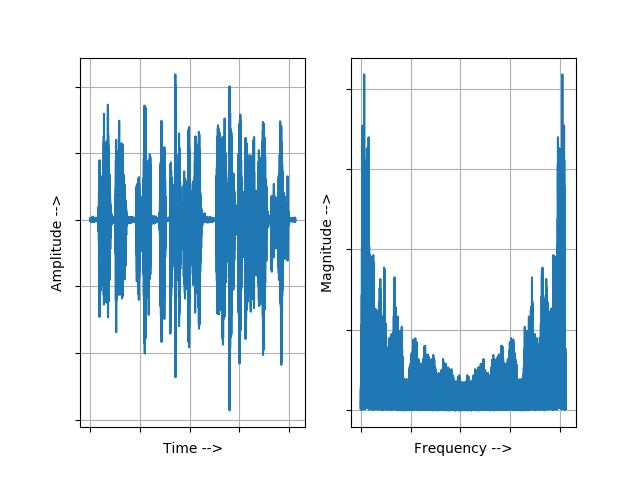
\includegraphics[width=0.85\columnwidth, height=0.40\columnwidth]{master_thesis_template/figs/fft.png}
    \caption[An example of DFT of a signal]{An example of time domain signal and its Fourier transformation.}
    \label{fig:speech_ex}
\end{figure}

\subsubsection{Short Time Fourier Transform}
The STFT of a time-frequency representation of a signal, in general, can be thought of as a compromise between a time and a frequency representation. It provides a way to simultaneously represent time as well as frequency components of a signal thereby providing a way to locate frequency events over time. The key idea behind STFT is to apply the FT locally over a signal using a window function. The window function is defined over an interval and provides a way to analyze the frequency content of a signal in a given segment.

Formally, the STFT of a signal $x\in\mathbb{R}^L$ with the window $w\in\mathbb{R}^L$, hop length $h\in\mathbb{N}$ and frequency steps $M\in\mathbb{N}$  is defined as:
\begin{equation}
    \hat{X}_w(a,b) = \sum_{l=0}^{L-1} x(l)\cdot w(l-nh)e^{-2\pi jab/M}
\end{equation}
for all $a\in\{0,...,N-1\}$ and $b\in\{0,...,M-1\}$ where $N$ is the number of time steps and $M$ is the frequency resolution. The hop length $h$ is a measure of redundancy, it is defined as the number of time steps between two consecutive window frames. Depending on the sampling frequency and hop length we can also express frequency step $a$ in Hz as $\Tilde{a} = a\cdot F_s/N$ and time step $b$ in seconds as $\Tilde{b}=b\cdot h/F_s$, where $F_s$ is the sampling rate of signal $x$. The entry $X(a,b)$ represents the Fourier coefficient present at the $a^{th}$ frequency and $b^{th}$ time step. 

Similar to FT we can also define the inverse transformation for STFT. For a given STFT matrix $\hat{X}_w$ under $\hat{w}$ an inverse short-time Fourier transform (ISTFT) is defined as:
\begin{equation}
    x(n) = \sum_{a=0}^{N-1} \sum_{b=0}^{M-1} \hat{X}_w(a,b)\cdot\hat{w}(n-ha)e^{2\pi jab/M}
\end{equation}

where $\hat{w}$ is an FT representation of window $w$. The window size controls the time-frequency resolution. A smaller window size in the time domain gives a good time resolution but a bad frequency resolution. Likewise, a large window size gives a better frequency resolution but a bad time resolution. The simultaneous time-frequency analysis is governed by the Heisenberg Uncertainty principle (\cite{gabor1946theory}). Improving the resolution in one domain affects the quality in the other domain and vice versa. Fortunately, the Gaussian window has minimum uncertainty and is a preferred choice for STFT. In this work, we use a type of Gaussian window called ``von Hann" window originally proposed by~\citet{harris1978use}. 

The STFT matrix has two parts: the magnitude and the phase information. Due to complexities in dealing with the phase information discussed in a later part in Section~\ref{subsec:phrecon}, the magnitude information is a preferable representation for machine learning tasks. The magnitude of an STFT matrix $\hat{X}_w(a,b)$ is defined as $\mathopen|\hat{X}_w(a,b)\mathclose|$.
In Figure~\ref{fig:time_freq_rep} (left side) gives an example of an STFT of a signal with a Gaussian window. The colored region in the spectrogram reflects the magnitude of the coefficients. A log transformation defined as $\ln(1+\mathopen|\hat{X}_w(a,b)\mathclose|)$ is commonly applied on the magnitude spectrogram to enhance the low magnitude coefficients. In Figure~\ref{fig:time_freq_rep} the middle part gives an example of the log transformation.


\subsubsection{Mel Spectrogram}
Human ears perceive the perceptual difference in sound quality based on the pitch of a signal. The pitch is a function of frequency and can be interpreted as the perceived frequency. The mel scale introduced by \cite{stevens1940relation} is a transformation which relates the real frequency to the perceived frequency also known as pitch. Various forms of mel functions have been proposed. One commonly used transformation is given by
\begin{equation}
    m = 2\,595 \log(1+\frac{f}{700})
\end{equation}
mapping the frequency $f$ (in Hz) to $m$ mels.
The magnitude spectrogram consists of different frequency bands. To perceive harmonics of each band it is essential that all bands have an equal resolution on the mel scale. This is achieved by applying a bank of overlapping triangular filters around the center frequency of each band. The Mel spectrogram is obtained by scaling the magnitude spectrogram to the mel scale and then passing it through the filterbanks. For further details on mel filterbanks, we refer to \cite{kopparapu2010choice}. Figure~\ref{fig:time_freq_rep} gives an example of a mel spectrogram and its comparison with the magnitude and log magnitude representation.
\begin{figure}
    \centering
    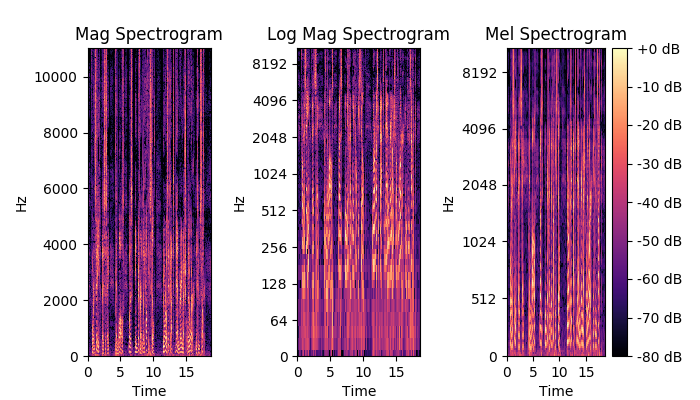
\includegraphics[width=0.95\columnwidth, height=0.40\columnwidth]{master_thesis_template/figs/freq_res.png}
    \caption[ Time frequency representation of signal]{Time frequency representation of signal illustrated in Figure~\ref{fig:speech_ex}. On the left is the magnitude spectrogram, in the middle is the log magnitude spectrogram and on the right is the mel spectrogram. For this example we use $1024$ point FFT with $75\%$ overlap, hanning window of size $1024$ and $128$ mel filters.}
    \label{fig:time_freq_rep}
\end{figure}

\subsection{Phase Reconstruction}
\label{subsec:phrecon}
The STFT representation $\hat{X}$ is a matrix of complex numbers. The squared magnitude of $\hat{X}$ is interpreted as an energy spectrum of a signal where each entry $(a,b)$ represents the energy of the signal at the frequency step $a$ and time step $b$. The angle of the STFT matrix $\hat{X}$ represents a phase of a signal at the frequency step $a$ and time step $b$. The phase representation consists of discontinuities at periodic components of a signal and it is not clear how this representation relates to the perceptual quality of sound. Thus, using the phase spectrogram increases the complexity of the analysis. As a consequence, the magnitude information of the STFT matrix is a preferable choice for various signal processing and machine learning tasks.

One problem with this choice is the consistency of the spectrogram under arbitrary transformations. The windowing in STFT is done with overlapping time frames. To preserve time-frequency dynamics any transformation on STFT should also take into account the proportion of the overlap. However, the methods in signal processing, as well as ML, often ignore this information. As a result, the modified magnitude spectrogram might not even have a valid time-domain reconstruction. Thus, to reconstruct a signal a crucial requirement is a right combination of phase information which in turn depends on the consistency of the spectrogram representation.

%However, for application like speech synthesis magnitude information is not sufficient to infer time domain signal.
\subsubsection{Spectrogram Consistency}
\label{subsec:spec_con}
As discussed previously any transformation applied to the magnitude spectrogram makes it difficult to reconstruct the time domain signal. In this work, we generate the spectrogram using a GAN. The details are discussed in the latter part of the thesis in Chapter~\ref{ch:unvc}. One central problem underlying the generation is the consistency of the spectrogram, that is to say, finding a unique time-domain signal from a generated spectrogram representation. In this part, we formally define the condition for consistency of the spectrogram.

Let $\mathbb{C}^{M N}$ be a space of complex matrices, $\mathbb{H}^L$ be a space of time-domain signals and $\mathbb{V}^{M N}$ be a space of consistent spectrograms. A consistent spectrogram $X\in\mathbb{V}^{MN}$  for some $x\in\mathbb{H}^L$ is a matrix which can be obtained by applying STFT on $x$. Since, $\mathbb{V}^{MN} \subset \mathbb{C}^{MN}$ implies $\exists  $W$\in\mathbb{C}^{MN}$ such that there is no unique reconstruction of $W$ in $\mathbb{H}^L$. Thus for any $W\in\mathbb{C}^{MN}$ to be a consistent spectrogram it should be in a null space of a linear transformation $\mathcal{F}$ defined as:
\begin{equation}
\label{eq:null}
    \mathcal{F}(W) = \text{STFT}(\text{ISTFT}(W)) - W
\end{equation}

The Figure~\ref{fig:spec_con} gives the geometrical illustration of the consistency of a spectrogram.

\begin{figure}
    \centering
    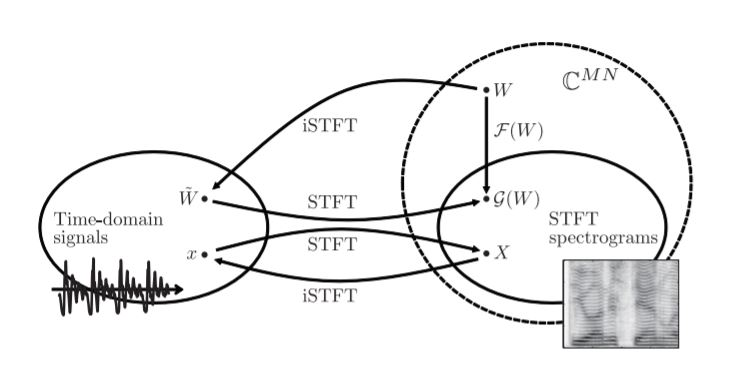
\includegraphics[width=0.55\columnwidth]{master_thesis_template/figs/spec_consistency.JPG}
    \caption[Spectrogram consistency]{An example of spectrogram consistency. Taken from~\cite{le2010fast}}
    \label{fig:spec_con}
\end{figure}
\subsubsection{Griffin Lim Reconstruction}
\label{subsec:gla}
The Griffin Lim algorithm (GLA) proposed by \citet{griffin1984signal} makes use of the consistency constraint to reconstruct the closest time-domain signal from a modified magnitude spectrogram. The GLA finds the phase for a magnitude spectrogram by projecting it into the null space of the operator $\mathcal{F}(W)$. Thus, it minimizes the projection error of Eqaution~\ref{eq:null} by iteratively projecting the signal across two domains i.e. from frequency to time and time to frequency. Under sufficient overlap of the window in the STFT operation, the GLA guarantees to reconstruct a solution approximating the corresponding time-domain waveform. Algorithm~\ref{alg:gla} further defines the GLA.

\begin{algorithm}
\caption{Griffin-Lim Algorithm}
\label{alg:gla}
\begin{algorithmic}[1]
\Procedure{GLA}{$\mathcal{\hat{M}}, n$} \Comment{Input: Modified Magnitude Spectrogram and number of training iterations}
\State $\phi_0$ $\leftarrow$ $\angle$ $\mathcal{N}(0,I)$ \Comment{Initial random phase in radians}
\State $\hat{\mathcal{S}}_o = \mathcal{\hat{M}}\cdot e^{-j\phi_o}$ \Comment{initial full spectrogram}
\For{i \text{in} \textbf{range (}1,n\textbf{)}} 
\State $\hat{\mathcal{S}}_i$ = $\text{STFT}\circ \text{ISTFT} (\hat{\mathcal{S}}_{i-1})$
\EndFor
\State x = $\text{ISTFT}$\{$\hat{\mathcal{S}_n}$\}
\State \textbf{return} x
\EndProcedure
\end{algorithmic}
\end{algorithm}

One problem often encountered with GLA is the low-quality reconstruction when dealing with high-quality sound signals. Many improvements of the GLA have been proposed. \citet{perraudin2013fast} formulate the phase reconstruction as an optimization problem and modify the conventional GLA. (\cite{pruuvsa2017noniterative}) utilized the phase magnitude relationship proposed by (\cite{auger2012phase}) and proposed a stable way to integrate the magnitude spectrogram at different scales. In this work, we limit our discussion to the GLA. For further details we refer to (\cite{perraudin2013fast},~\cite{le2010fast},~\cite{jaganathan2015phase}).

\section{Deep Generative Models}
\label{sec:dgm}
In this section, we build our discussion around deep generative models. We will start with a gentle introduction to deep learning in Section~\ref{subsec:dl}. We will then briefly discuss about generative models in Section~\ref{subsec:gm} followed with a detailed discussion on generative adversarial networks (GANs) in Section~\ref{subsec:gan}. Further, in Section~\ref{subsec:train_gan} we look at the training procedure of GAN, its convergence propoerties in Section~\ref{subsec:gan_itp} and evaluation measures in Section~\ref{subsec:eval_metrics}.Finally, we conclude our discussion with other GMs, VAE in Section~\ref{subsec:vae}, cycleGAN in Section~\ref{subsec:cgan} and unsupervised image-to-image translation in Section~\ref{subsec:unit_gan}. 
\subsection{A short introduction to Deep Learning}
\label{subsec:dl}
In recent years deep learning (DL) has emerged as a popular choice for modeling various artificial intelligence (AI) tasks ranging from object recognition in computer vision to language models in NLP. DL works on the principle of building a solution to a complex problem by decomposing it into simpler ones which reduce the complexity of the problem and provides insights to model non-linear dynamics of data. 

\citet{Goodfellow-et-al-2016} outline DL as:
\textit{``A way to allow computers to learn from experience and understand the world in terms of a hierarchy of concepts, with each concept defined through its relation to simpler concepts. By gathering knowledge from experience, this approach avoids the need for human operators to formally specify all the knowledge that the computer needs. The hierarchy of concepts enables the computer to learn complicated concepts by building them out of simpler ones. If we draw a graph showing how these concept defined as the decomposition of complex concepts into simple ones and the recombination into new complex concepts. An algorithm therefore has to establish a hierarchy of concepts. A visualization of this hierarchy would be a multi-layered graph, that can be called deep in a graph theory context."}

\subsubsection{Artificial Neural Network}
\label{sub:ann}
An artificial neural network (ANN) is a learning model inspired by the working of biological neurons. It consists of an arbitrary number of small computational units called artificial neurons and solves a learning problem by modeling the strength of the connection between them. This nature of ANNs allows them to model functions of arbitrary complexity and thus classifies them as universal approximators (\cite{hornik1989multilayer}).

We start our discussion with the basic form of an ANN commonly referred as \emph{perceptron}. The \emph{perceptron} uses a single neuron to approximate a function. Following \citet{mitchell1990machine} we define the perceptron model. For an input $x\in\mathbb{R}^D$ and the parameterized function $f:x\rightarrow y$ defined as $f(x;w,b)=w^Tx+b$ where  $y\in\mathbb{R}$ is an output score, $w\in\mathbb{R}^D$ is a weight parameter and $b\in\mathbb{R}$ is a bias term. For a binary classification task the output $f(x;w,b)$ is further passed through the decision function also referred as
\emph{activation function} formally given by Equation~\ref{eq:act_fun}. 
\begin{equation}
\label{eq:act_fun}
  \hat{y}= 
\begin{cases}
    1,& \text{if } f(x;w,b)> 0\\
    0,              & \text{otherwise}
\end{cases}  
\end{equation}

The initial parameters $(w,b)$ are set to zero. At every step of learning the output, $y$ is computed and the parameters are adjusted based on the mean-squared-error between target and predicted output. One major limitation of the \emph{perceptron} is that it cannot model non-linear relations, as for instance, \texttt{XOR} function. 

The \emph{Multilayer perceptron} (MLP) is a class of ANNs which unlike the perceptron uses multiple neurons over several layers to approximate the unknown function. The interconnected neurons form a hierarchical network which allows to model a function of arbitrary complexity. Also, there are various families of activation functions which can further improve the learning process.

Formally, a MLP can be considered as a chain of functional maps applied on data to unravel the non-linearities over several layers of the hierarchy. Let $L$ be the number of layers, $x\in\mathbb{R}^d$ be an input representation, for a layer $l$: $d_l\in\mathbb{N}$ be number of neurons, $v^{l}$ be an input representation, $u^{l}$ be an output representation, $f_l:\mathbb{R}^{d_{l-1}}
\rightarrow\mathbb{R}^{d_{l}}$ be a transformation mapping $u^{l-1}$ to  $u^l$, let $\theta^{l-1,l}=\{w^{l-1,l},b^{l-1,l}\}$ be parameters connecting layer $l-1$ to $l$ and $\sigma^{l}$ be an activation function, then the output of the MLP $f(x)$ is defined as:
\begin{equation}
\label{eq:mlp}
\begin{aligned}
    v^{0}(x) = x\\
    v^{l}(x) = u^{l-1}(x)\\
    u^{l}(x) = \sigma^l(f^{l}(v^{l},\theta^{l-1, l}))\\
    f^{l}(v^{l},\theta^{l-1, l}) = w^{l-1, l}\cdot u^{l}+b^{l-1,l}\\
    f(x) = u^{L}\circ u^{L-1}\circ...\circ u^{1}\circ u^{0}(x)
\end{aligned}
\end{equation}

The MLPs are efficient in modeling any class of functions. However, it is difficult to train MLPs with a large number of neurons in the hidden layers. This is because each neuron connects to all the neurons of the previous layer. As a result the number of parameters increase significantly making learning infeasible. Another issue with MLPs is that they are permutation invariant i.e. if the feature space is shuffled the output of the network is still the same. As a result, it fails in modeling the spatial correlation in data. For further details we recommend readers to refer to \citet{Goodfellow-et-al-2016}.


\subsubsection{Convolutional Neural Network}
\label{sub:cnn}
Convolutional neural networks (CNN) (\cite{lecun1995convolutional}) take the inspiration from the receptive-field of the visual cortex. In the visual cortex, neurons form local regions form receptive-field a.k.a feature-maps where neurons respond selectively to various attributes of visual input. The CNN exploits this idea to implement local feature-maps which by weight sharing learns different levels of abstraction from a given input.  

A convolution is a linear operator which takes two functions as an input and provides another function as an output. This composition is defined to capture the \emph{cross-correlation} between the two functions. Formally, for an input $x\in \mathbb{R}^N$ and a receptive field in $w\in \mathbb{R}^K$ the convolution operator is defined as:
\begin{equation}
\label{eq:conv}
    y(n) = (x \ast w)(n)  = \sum_{k=0}^{K} x(k)\cdot w(n-k)
\end{equation}
where $n\in\{0,...,N+K-1\}$. Likewise, a convolution operator can be extended to multidimensional input $x\in\mathbb{R}^{M_1\times M_2\times ...M_d}$. For a more comprehensive explanation we refer to \citet{Goodfellow-et-al-2016}.

The CNN uses a convolutional operator to apply a parametric transformation on the input representation. Thus, learning parameters which are effective in capturing spatial or temporal correlations in the data. For an input $x\in\mathbb{R}^{m\times n \times c}$, the convolutional layer  $l\in L$ with filter maps $w\in\mathbb{R}^{k_l \times k_l \times c_{l-1}}$ in CNNs is a three step operation: (i) Apply the convolutional operator $f_l:\mathbb{R}^{m_{l-1}\times n_{l-1}\times c_{l-1}} \rightarrow\mathbb{R}^{m_{l}\times n_{l}\times c_{l}}$ to obtain an intermediate output. (ii) Apply the activation function $\sigma^{l}$ and (iii) Apply the pooling operation $g_l^d:\mathbb{R}^{m_{l-1}\times n_{l-1}\times c_{l-1}}\rightarrow \mathbb{R}^{m_{{l-1}/d}\times n_{{l-1}/d}\times c_{l-1}}$ to downsample the output of activations, where $c_0 = c$ is number of input channels, $m_l\times n_l \times c_l$ is the shape of the output of $l^\text{th}$ layer and $\sigma^l$ is the activation function used in $l^\text{th}$ layer.

Depending on the design choice, the step (iii) can also be omitted sometimes. An optimal choice of the number of filter maps and its size is a hyperparameter optimization problem and is usually decided by heuristics or grid search. A stack of convolutional layers followed by some layers of an MLP is a preferrable design choice of CNNs and have shown a lot of success particularly in computer vision tasks like object recognition (\cite{krizhevsky2012imagenet}, ~\cite{donahue2014decaf}). However, for tasks like super-resolution or object localization where the output is essentially in a spatial domain a fully convolutional (FCN) approach is a preferred design choice. The FCNs learn a path from pixels in the first layers to the pixel in the deeper layers thus preserving point to point correspondence and produce an output in the spatial domain. 

%In addition,  $W^{l}_{l-1}$ is defined for every receptive field $q\in Q$ as a local region $W^{l, q}_{l-1}\in\mathcal{R}^{k\times k\times c}$, where $k$ is the size of receptive field, $c$ is the number of channels in an input and $m\times n$ is the dimensionality of each input channel.

%For an input $x\in\mathcal{R}^{m\times n \times c}$, for a layer $l$: $V^{l}$ be an input representation, $U^{l}$ be an output representation, and filter maps $w\in\mathcal{R}^{k_l \times k_l \times c_{l-1}}$

%$f_l:\mathcal{R}^{d_{l-1}}\rightarrow\mathcal{R}^{d_{l}}$ be a transformation mapping $U^{l-1}$ to  $U^l$, $\theta^{l-1,l}=\{W^{l-1,l},b^{l-1,l}\}$ be parameters connecting layer $l-1$ to $l$ and $\sigma^{l}$ be a activation function


 %the convolution operator for arbitrary layer $l$ with $c_l$ kernels is defined as:
%\begin{equation}
%    \begin{aligned}
%    V^{0}_{c_0}(x) = x\\
%    V^{l}_{c_l}(x) = U^{l-1}_{c_l}(x)\\
%    U^{l}_{c_l}(x) = \sigma^l(f^{l}(V^{l}_{c_l},\theta^{l-1, l}_{c_l}))\\
%    f^{l}(V^{l}_{c_l},\theta^{l, l-1}_{c_l}) = W^{l-1, l}_{c_l}*_{c_l} U^{l}_{c_l}+b^{l-1,l}_{c_l}\\
%    f(x) = U^{L}_{c_L}\circ U^{L-1}_{c_{L-1}}... U^{1}_{c_1}\circ U^{0}_{c_0}(x)        
%    \end{aligned}
%\end{equation}


\subsubsection{Residual Networks}
\label{sub:resnet}
The training of deep neural networks is difficult. The increasing depth results in the saturation of the performance followed with a rapid degradation. The residual networks (ResNets) introduced by \citet{he2016deep} address this problem by proposing skip identity connections. The key idea behind ResNets is that for every shallow network there is a corresponding deep network with identity mappings. The ResNets introduce \emph{skip identity connections} to learn a change in a function rather than a function itself which is a relatively simpler learning task (\cite{he2016identity}). For an input $x$, the intermediate output $u^l(x,\theta^l)$ of layer $l$ the output of the residual block is defined as:
\begin{equation}
\label{eq:res}
    u^{l+1}(x,\theta^{l+1}) =  u^{l}(x,\theta^l) + \mathcal{F}^l(u^{l}(x,\theta^{l}), \theta^{l+1})
\end{equation}



%\subsubsection{Batch Normalization}
%\ref{sub:bnorm}
%Batch normalization (BN)~\cite{??} provides ways 
%\subsubsection{Instance Normalization}

\subsubsection{Optimization in Deep Learning}
\label{sub:mll}
The learning of parameters in NNs is formulated as an optimization problem. In this section we will discuss in the context of supervised learning where we have associated labels for data points. Our discussion follows from \citet{mitchell1990machine}.

Let $\mathcal{D}=(\mathcal{X},\mathcal{Y})=\{(x_1,y_1),...,(x_N,y_N)\}$ be a set of $N$ independent and identically distributed (i.i.d) data points sampled from the data probability distribution $P_{(x,y)\sim \mathcal{X},\mathcal{Y}}(x,y)$, where $x_i\in\mathbb{R}^d$ is a feature representation of $i^\text{th}$ sample and $y_i\in\mathbb{R}$ is an associated label. We split $\mathcal{D}$ into two sets namely the \emph{training} and the \emph{test} set given as:
$\mathcal{D}_\text{train}=(\mathcal{X}_\text{train},\mathcal{Y}_\text{train})=\{(x_1,y_1),...,(x_M,y_M)\}$, $\mathcal{D}_\text{test}=(\mathcal{X}_\text{test},\mathcal{Y}_\text{test})=\{(x_{M+1},y_{M+1}),...,(x_N,y_N)\}$. In supervised learning our objective is to learn a model represented as a parametric function $f:\mathcal{X}_\text{train}\rightarrow\mathcal{Y}_\text{train}$ and later use it to make prediction on the test set as $f:\mathcal{X}_\text{test}\rightarrow\mathcal{Y}_\text{test}$. For a parametric function $f$ we define a performance measure a.k.a. loss function $L:\mathcal{X}\times\mathcal{Y}\times\mathbb{R}\rightarrow[0,\infty)$ which gives the estimate of quality of the model prediction $\mathcal{L}(x,y,f(x))$ for a sample $(x,y)\in\mathcal{D_\text{train}}$. 

The learning can now be interpreted as an optimization problem to learn a function $f$ which minimizes the expected value of the loss function a.k.a. risk of a function $f$ expressed as:
\begin{equation}
    R_f = \int_{\mathcal{X}\times\mathcal{Y}}L(x,y,f(x))p(x,y)dydx
\end{equation}

For a model to generalize well on unseen samples we need an optimal parametric function $\hat{f}$ which has minimum loss on test points:
\begin{equation}
    \hat{f} = \argmin_f \frac{1}{N-M} \sum_{i={M+1}}^N L(x_i,y_i,f(x_i))
\end{equation}

A main problem with this estimate is that we do not know $P_{(x,y)\sim \mathcal{X},\mathcal{Y}}(x,y)$. 
However, under an assumption data points are i.i.d., we can alternatively minimize the empirical risk:
\begin{equation}
    \hat{R}_f =  \frac{1}{M} \sum_{i=0}^M L(x_i,y_i,f(x_i))
\end{equation}

for a fixed $f$ if $M\rightarrow\infty$ then $\hat{R}_f\rightarrow R_f$. This form of optimization is known as \emph{empirical risk minimization} (ERM).  

The optimization of deep learning comes with various challenges: (i) The deep learning optimization problems are solved using gradient descent-based methods. As a result, a certain choice of the loss function is also not feasible. For example, a $0$-$1$ loss used in the classification task is not differentiable. 
(ii) The ERM principle minimizes the expected value of the training loss. An associated problem is that a model with a sufficiently large number of parameters can memorize the training data with empirical risk $\hat{R}_f \approx 0$ and fail to generalize on the testing data resulting in overfitting. 
(iii) The learning task can be too complex for a model or a model is not expressive enough due to limited number of parameters. This results in high empirical risk indicating that the model is not properly learning thus causing underfitting. 

To overcome the above issues the deep learning models are trained in a slightly different approach with certain tricks. For instance, in a classification problem instead of using $0$-$1$ loss, we use a proxy or surrogate loss like the log-likelihood of the correct class. We use regularization to prevent the model from being too complicated and avoid overfitting. Early stopping is another alternative to prevent overfitting. For comprehensive details we recommend \citet{Goodfellow-et-al-2016}.

\subsubsection{Gradient based Optimizers}
\label{sub:gbl}
The optimization problem of deep neural networks is solved using a gradient-based method. The most commonly used gradient-based algorithm is called gradient descent (GD). The key idea behind GD is to start with an initial configuration of parameters $\theta_0$ and iteratively update the parameters in the negative direction of the gradient of a function to be optimized. 

Formally, consider a multi-dimensional continuous function $f:\mathbb{R}^n\rightarrow\mathbb{R}^m$ with parameters $\theta\in\mathbb{R}^{n\times m}$. The gradient of a function $f(\theta)$ with respect to parameters $\theta$ is defined as:
\begin{equation}
    \label{eq:jacob}
    \nabla_{\theta} f = \begin{bmatrix}
    \frac{\partial f}{\partial \theta_{00}} & \dots  & \frac{\partial f}{\partial \theta_{0n}} \\
    \vdots & \ddots & \vdots \\
    \frac{\partial f}{\partial \theta_{m0}} & \dots  & \frac{\partial f}{\partial \theta_{mn}}
\end{bmatrix}
\end{equation}

The iterative update of a GD is defined as:
\begin{equation}
    \label{eq:gradupdate}
    \theta_{n+1} = \theta_{n} - \eta \nabla_{\theta}f(\theta)
\end{equation}

where $\eta\in\mathbb{R}^+$ is the learning rate which controls the rate of convergence. In the case of NNs $f:\mathbb{R}^{d}\rightarrow \mathbb{R}$ is a function computed by taking the average of loss function over all training samples:
\begin{equation}
    f(\theta) = \frac{1}{M}\sum_{i=0}^M\mathcal{L}(x_i, y_i;\theta)
\end{equation}

where $(x_i,y_i)\in\mathcal{D}_\text{train}$. For a large dataset computing the gradient-update for all training samples is computationally infeasible as it requires summation over all samples. This issue is addressed with the stochastic update rule where gradients are updated for a randomly sampled batch of samples from the data set. This makes learning tractable and also results in faster convergence. Algorithm~\ref{alg:grad_des} gives describes the pseudocode of stochastic-gradient-descent.

\begin{algorithm}
\caption{Stochastic Gradient Descent}
\label{alg:grad_des}
\begin{algorithmic}
\State \textbf{Initialize} Learning rate: $\eta$, Model parameters: $\theta$
\Repeat
\State Randomly sample minibatch of samples $\{(x^{(1)},y^{(1)}),...,(x^{(m)},y^{(m)})\}\sim p_\text{data}$ 
\State Compute Mini-batch gradient $\theta_\text{grad} \leftarrow \frac{1}{m}\sum_{i=0}^M \nabla_{\theta}\mathcal{L}(x^{(i)}, y^{(i)},\theta)$
\State Update the parameters $\theta\leftarrow\theta - \eta \theta_\text{grad}$
\Until{Convergence}
\State
\end{algorithmic}
\end{algorithm}
In general, the optimization of deep neural networks is often difficult due to the complexity of the curvature of the loss function mainly introduced by a large number of network parameters. There are various other learning methods introduced as an improvement over SGD. \citet{qian1999momentum} introduced momentum with an idea of a ball with mass moving downhill analogous to curvature of the loss function. \citet{duchi2011adaptive} introduced an adaptive learning rate of each parameter allowing slower update for frequently occurring features. \citet{kingma2014adam} introduced Adam an optimizer which utilizes momentum as well as the adaptive learning rate.
We avoid a detailed discussion of all methods. For a detailed discussion, we refer to \citet{Goodfellow-et-al-2016}.


%or a given input $\{(x_1,y_1),...,(x_N,y_N)\}\in\mathcal{D}$, where $x_i\in\mathcal{R^D}$ is an input representation of $i^\text{th}$ sample of data 



\subsection{Generative Models}
\label{subsec:gm}
The GMs deal with the estimation of the probability distribution of data. 
More specifically, consider $p_\text{data}$ to be a true data distribution, $D_\text{data}$ be a set of training samples. The objective of generative model is to learn a distribution $p_\text{model}$ using $D_\text{data}$ such that $p_\text{model}$ is a good approximation of $p_\text{data}$. Such an estimate provides the description of data and thus can be used to generate new samples.

Following \cite{goodfellow2016nips} we characterize GMs as: (i) explicit density models, a class of model which learn $p_\text{model}$ explicitly. The common models in this class are: Restricted Boltzmann Machines (RBMs) (\cite{salakhutdinov2007restricted}), Sigmoid Belief Networks (SBNs) (\cite{hinton2009deep}), Deep Boltzmann Machines (DBMs) (\cite{salakhutdinov2009deep}). One main problem in designing this class of model is the computational intractability. For details refer to (\cite{salakhutdinov2015learning},~\cite{goodfellow2016nips}).
(ii) implicit density models, a class of model which learns to generate samples from $p_\text{data}$ without explicitly defining a density function. Some common models in this class are generative stochastic networks (GSNs) (\cite{bengio2014deep}), generative adversarial networks (GANs) (\cite{goodfellow2014generative}), etc.

\subsubsection{Maximum Likelihood Principle}
\label{sub:mll}
The above class of GMs are commonly solved using the maximum likelihood principle.
Let $\mathcal{X}=\{x_1,...,x_N\}$ be a set of training samples, $f(x;\theta)$ be a parametric model that provides an estimate of the data distribution $p_\text{data}$ using a model distribution $p_\text{model}$.  Our goal is to find the configuration of parameters $\theta$ which gives the best estimate of $p_\text{model}$ approximating $p_\text{data}$. Using the maximum likelihood principle the best parameters $\hat{\theta}$ is given by Equation~\ref{eq:mll}. To further ease the optimization points are sampled from an i.i.d. distribution and the optimization is solved in the log space.
\begin{eqnarray}
     \label{eq:mll}
    \hat{\theta} & = & \argmax_{\theta}p_{model}(\mathcal{X};\theta)\\
     &= & \argmax_{\theta} \prod_{i=0}^N p_{model}(x_i;\theta)\\
     &= & \argmax_{\theta} \sum_{i=0}^N \log p_{model}(x_i;\theta)
\end{eqnarray}

Figure~\ref{fig:mll} gives an example of a maximum-likelihood principle.
\begin{figure}
    \centering
    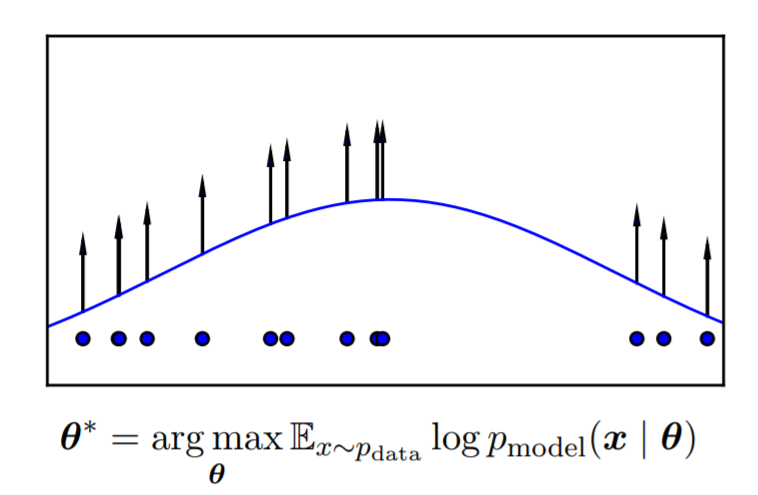
\includegraphics[width=0.45\columnwidth]{master_thesis_template/figs/mll.PNG}
    \caption[Maximum Likelihood Principle]{An illustration of a maximum likelihood principle shows how different data points push up different part of the density function. The maximum likelihood principle takes samples from the training set and then pushes up the probability that a model assigns to those points. Taken from \citet{goodfellow2016nips}}
    \label{fig:mll}
\end{figure}

\subsection{Generative Adversarial Networks}
\label{subsec:gan}
Learning to sample from high dimensional probability distribution $p_\text{data}$ is complicated and often an intractable process. However, sampling from a simple distribution like a Gaussian is well studied and computationally efficient. 
The key idea behind GANs (\cite{goodfellow2014generative}) is to take samples from simple distribution and apply a non-linear parametric transformation to get samples from the high dimensional complex distribution. This learnable transformation is optimized in an adversarial setting.

A GAN consists of two networks namely generator $\mathcal{G}$ and a discriminator $\mathcal{D}$. Consider $p(z)$ to be a prior noise distribution, $\mathcal{X}$ be a set of training samples drawn from data distribution $p_\text{data}$. The network $\mathcal{G}$ transforms samples from noise distribution $z\sim p(z)$ to samples in model distribution $\mathcal{G}(z;\theta_g)$. The network $\mathcal{D}$ takes an input sample $x$ and estimates the probability $\mathcal{D}(x;\theta_d)$ of sample $x$ being drawn from $\mathcal{X}$. Thus a discriminator $\mathcal{D}$ works as a binary classifier to discriminate between real samples in $\mathcal{X}$ and generated samples $\mathcal{G}(z;\theta_g)$. The objective of generator $\mathcal{G}$ is to generate samples which are similar to real samples and thus can effectively fool the discriminator at the task of classification. 

\subsection{How to train a GAN?}
\label{subsec:train_gan}
The objective of the generator and discriminator can be interpreted as a minimax game where the generator tries to minimize the gain of the discriminator and the discriminator tries to maximize its gain. Formally, a minimax game between $\mathcal{G}$ and $\mathcal{D}$ is expressed by Equation~\ref{eq:gan_loss}. The two players $\mathcal{G}$ and $\mathcal{D}$ are represented by a parametric function and are fully differentiable with respect to their input as well as parameters and thus are typically modeled by neural networks.

\begin{equation}
    \label{eq:gan_loss}
    \min_{\mathcal{G}} \max_{\mathcal{D}} V(\mathcal{D}, \mathcal{G}) = \mathbb{E}_{x\sim p_\text{data}} [\log \mathcal{D}(x)] + \mathbb{E}_{z\sim p(z)} [\log (1 - \mathcal{D}(\mathcal{G}(z))]
\end{equation}

The differentiable nature of $\mathcal{G}$ and $\mathcal{D}$ allows solving the optimization using gradient-based methods. Since the input of one depends on the output of other the optimization is solved in two steps of gradient updates, first updating the parameters of $\theta_g$ and then updating $\theta_d$. Algorithm~\ref{alg:train_sgd_gan} further illustrates the learning of $\mathcal{G}$ and $\mathcal{D}$. Figure~\ref{fig:gan_train} gives a geometric illustration of GAN training.

\begin{algorithm}
    \caption[Minibatch training of a GAN]{Minibatch stochastic gradient descent training of GAN (\cite{goodfellow2014generative}). For each update of the generator  we update the discriminator k number of times, where k is the hyperparameter}
    \label{alg:train_sgd_gan}
    \begin{algorithmic}
        \For{number of iterations}
        \For{k steps}
            \State Sample minibatch of m noise samples from prior $\{z^{(1)},..., z^{(m)}\}\sim p_z(z)$.
            \State Sample minibatch of m samples from data distribution $\{x^{(1)},...,x^{(m)}\} \sim p_\text{data}$.
            \State Update the parameters of the discriminator by ascending the stochastic gradient on a minibatch:
            \State $\nabla_{\theta_d} \frac{1}{m} \sum_{i=1}^m [\log \mathcal{D}_{\theta_d}(x^{(i)}) 
             + \log (1 - \mathcal{D}_{\theta_d}(z^{(i)}) )]$
        \EndFor
        \State Sample minibatch of m noise samples from prior $\{z^{(1)},..., z^{(m)}\}\sim p_z(z)$.
        \State Update the generator by descending the stochastic gradient on a minibatch:
        \State $\nabla_{\theta_g} \frac{1}{m}  \sum_{i=1}^m [ \log (1 - \mathcal{D}_{\theta_d}(\mathcal{G}_{\theta_g}(z^{(i)}) )]$
        \EndFor
    \end{algorithmic}
\end{algorithm}

At each step of training, the cost of one player depends on the decision of the other one. However, both players have no control over the strategy of each other. This results in a zero-sum game where the loss of one player is equivalent to the benefit of the other one. If both players are optimal then there exists an equilibrium between them referred to as Nash Equilibrium. In the NN setting of a GAN, the optimization problem of both $\mathcal{G}$ and $\mathcal{D}$ is non-convex and the only plausible solution is a local minimum which implies an existence of a local Nash Equilibrium a state in which cost of $\mathcal{G}$ is minimal w.r.t parameters $\theta_g$ and of $\mathcal{D}$ is minimal w.r.t. parameters $\theta_d$ (\cite{ratliff2013characterization}).

\subsection{GAN: An Information Theoretic Perspective}
\label{subsec:gan_itp}
In this section, we will study the convergence properties of Algorithm~\ref{alg:train_sgd_gan}. Consider $p_\text{data}$ to be the probability distribution of the data and $p_\text{g}$ to be the probability distribution learned by the generator $\mathcal{G}$. We want to measure how well the probability distribution $p_\text{g}$ approximates the distribution $p_\text{data}$. To study the convergence we will assume that the $\mathcal{G}$ and $\mathcal{D}$ networks are of infinite capacity. We will first introduce Kullback-Leibler (KL) Divergence and Jensen Shannon Divergence and will then continue our discussion of optimality.

\subsubsection{Kullback-Leibler Divergence}
\label{subsec:kld}
The KL
divergence (\cite{kullback1951information}) is a measure of discrepancy between two probability distributions. From an information theory point of view, a KL-divergence between two probability distributions $P$ and $Q$ is a measure of an extra number of bits required to code samples from $P$ when using a code of samples from $Q$. It tells us how much information is lost when $Q$ is used to approximate $P$. Formally, it is defined as:
\begin{equation}
    \label{eq:kld}
    D_{KL} (P || Q) = \mathbb{E}_{x\sim P} \log \frac{P}{Q}
\end{equation}

The KL divergence is a non-negative quantity and is equal to zero if and only if $P=Q$. It is not a proper metric as it is asymmetric and does not obey the triangle inequality.

%\begin{equation}
%    \label{eq:kld}
%    D_{KL} (p_\text{data} || p_\text{g}) = \mathbb{E}_{x\sim p_\text{data}} \log \frac{p_\text{data}}{p_\text{g}}
%\end{equation}

\subsubsection{Jensen-Shannon Divergence}
\label{subsec:jsd}
Jensen–Shannon divergence (JSD) is another common measure of similarity between two probability distributions. It is symmetric and a smoothed variant of the KL divergence and is defined as:
\begin{equation}
    \label{eq:jen_shan}
    JSD(P,Q) = KL(P||M) + KL(Q||M)
\end{equation}
where $M = \frac{P+Q}{2}$. The choice of $M$ as the average of $P$ and $Q$ further gives an upper bound on the divergence. In an information theory sense, JSD is regarded as the mutual information between a mixture distribution of $P$ and $Q$ and a random variable indicating the switch between $P$ and $Q$ to produce the mixture.

\subsubsection{Optimality of minimax}
The optimal solution to $V(G,D)$ corresponds to finding a parameter configuration $\theta_g$ that minimizes the objective and $\theta_d$ that maximizes the objective. The optimal discriminator $\mathcal{D}$ for a fixed $\mathcal{G}$ is given by:
\begin{equation}
    \label{eq:opt_gan}
    D_{G}^{\ast}(x) = \frac{p_\text{data}(x)}{p_\text{data}(x) + p_\text{g}(x)}
\end{equation}

For an optimal discriminator the optimization function can be formulated as:
\begin{flalign}
%\begin{aligned}
    C(G) = & \max_D V(G,D) \\
     =&  \mathbb{E}_{x\sim p_\text{data}} [\log \mathcal{D}^\ast(x)] + \mathbb{E}_{z\sim p(z)} [\log (1 - \mathcal{D}^\ast(\mathcal{G}(z))]\\
     =& \mathbb{E}_{x\sim p_\text{data}} [\log \frac{p_\text{data}(x)}{p_\text{data}(x) + p_\text{g}(x)}] + \mathbb{E}_{z\sim p(z)} [\log \frac{p_g(x)}{p_\text{data}(x) + p_\text{g}(x)}]\\
%\end{aligned}
\end{flalign}

For $p_g = p_\text{data}$ the loss function $ C(G)$ can further be expressed as:
\begin{equation}
    C(G) = -\log 4 + 2\cdot JSD(p_\text{data} || p_g)
\end{equation}

As discussed in Section~\ref{subsec:jsd} the $JSD$ is non-negative and takes a minimum when the two distributions are equal. The optimization problem has a global optimum when $p_g = p_\text{data}$ i.e. with an infinite capacity the generative network can perfectly model the data distribution. Thus, in the training process, the optimal discriminator aims at estimating the ratio of probability densities as given in Equation~\ref{eq:opt_gan} and the optimal generator aims at minimizing the $JSD$ between $p_g$ and $p_\text{data}$.
%Thus solution is a saddle point where both generator and discriminator are optimal. The optmi


\begin{figure}
    \centering
    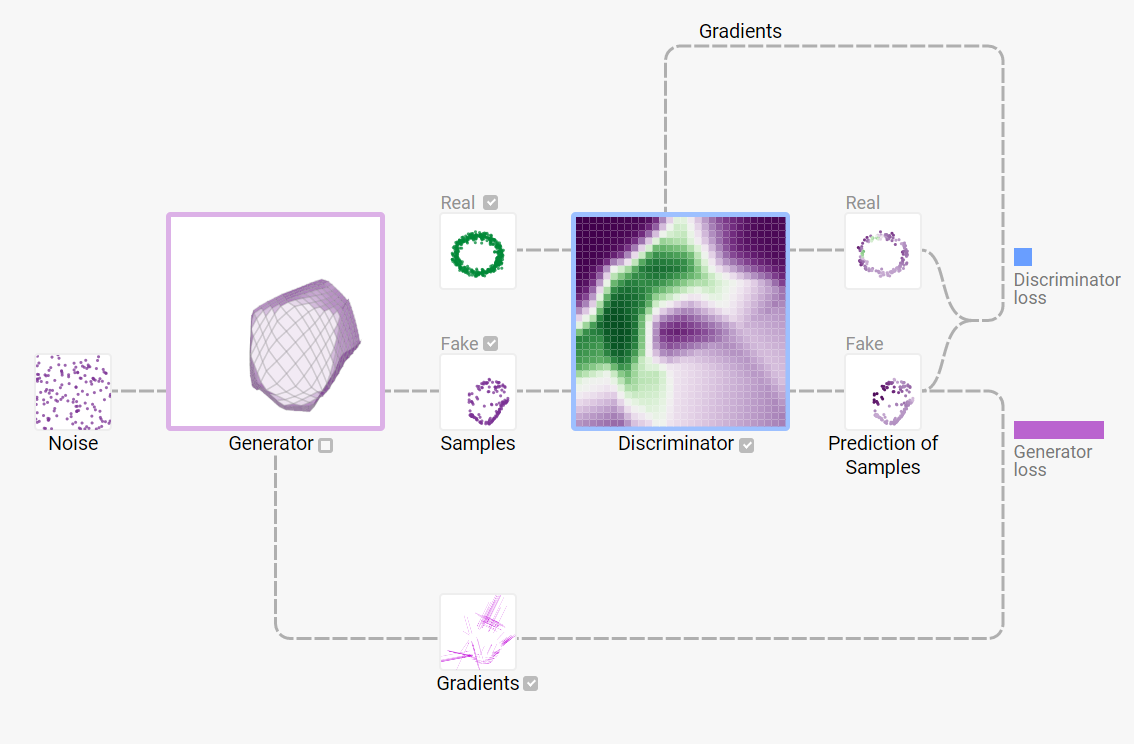
\includegraphics[width=0.75\columnwidth]{master_thesis_template/figs/gan_training.PNG}
    \caption[A geometric illustration of GAN training.]{A geometric illustration of GAN training. Generator learns to transform samples from a simple noise distribution $\mathcal{N}(0,1)$ to complex data distribution. Taken from~\cite{kahng2018gan}}
    \label{fig:gan_train}
\end{figure}
\subsubsection{Challenges in GAN training}
\label{subsec:ch_gan_train}
The training of GANs requires finding an equilibrium between generator and discriminator. At each step, $\mathcal{G}$ and $\mathcal{D}$ try to undo the progress of each other which makes it difficult to monitor their convergence. Thus, the training of GANs is often associated with instability. The two main problems are: (i) Oscillatory behavior across modes: This is a situation where the generator progressively switches from generating one kind of sample to another without reaching an equilibrium condition. (ii) Mode collapse: In mode collapse the generator starts mapping multiple latent noise representations to a single point in the data distribution. The more commonly encountered form of a model collapse in training of GANs is known as partial mode collapse which occurs when the generator maps only to a smaller set of training examples resulting in a low diversity of generated samples. This is further explained by the asymmetric nature of minimax that is to say:
\begin{equation}
\min_G \max_D V(G,D) \neq \max_D \min_G V(G,D)
\end{equation}
In the minimax situation the optimal generator draws sample from the data distribution. 
\begin{equation}
    G^\ast = \min_G \max_D V(G,D)
\end{equation}

In the case of maxmin, the optimization is first for generator and then discriminator. As a result, it maps every noise distribution to a single data sample. The update methods do not differentiate between minimax and maxmin. As a result in some cases the optimization turns out to solve the maxmin resulting in the mode collapse. The severity of mode collapse also depends on the diversity of training data. It is more common when training data consists of samples of only a few modes. 

\subsection{Evaluation of GANs}
\label{subsec:eval_metrics}
Over the past few years, various improvements have been proposed for GAN training (e.g.~\cite{karras2017progressive},~\cite{arjovsky2017wasserstein},~\cite{petzka2017regularization}). Despite all the improvements, the evaluation and comparison of models is still a difficult task. In this work, we use two widely accepted measures namely the inception score (\cite{salimans2016improved}) and the Fr\'echet inception distance (\cite{heusel2017gans}). 

To evaluate the quality of the generated samples we compute Inception Score (IS) and Fr\'{e}chet Inception Distance (FID). In the following section, we will look into the formalism of IS and FID. For the evaluation of generated samples, we use a held out set of $40$ speakers. 

\subsubsection{Inception Score}
\label{subsec:inception_score}
The IS (\cite{salimans2016improved}) was introduced as a measure to capture the diversity of generated samples. It was originally proposed for the evaluation of GANs trained to generate images. The two key ideas behind the IS are: (i) an image $x$ which contains a meaningful object has a low entropy of the label distribution $p(y|x)$ and (ii) for the high diversity in generated samples the marginal distribution $\int p(y|x=G(z)) dz$ should have a high entropy. By combining the two ideas IS is defined as:
\begin{equation}
    \text{IS} = \exp^{\mathbb{E}_{x\sim p_g} [KL (p(y|x)||p(y))]}
\end{equation}


where $p_g$ refers to the generated distribution and $\exp$ is done for scaling the scores to comparable range. For $m$ samples and $K$ classes the term $\mathbb{E}_x [KL (p(y|x)||p(y))]$ is defined as:
\begin{equation}
    \mathbb{E}_x [KL (p(y|x)||p(y))] = \frac{1}{m}\sum_{i=0}^{m-1}\sum_{k=0}^{K-1}p(y_k|X_i)\log(\frac{p(y_k|X_i)}{p(y_k)})
\end{equation}

%$p(y_k)$ 
 
The intuition behind the IS also follows for speech samples. If the generated sample contains utterance properties of a unique speaker the conditional label distribution should have a low entropy. Likewise, for the diversity in speakers in generated samples, the marginal $\int p(y|x=G(z))) dz$ should have a high entropy.
For the IS we use our speaker detection network discussed in Section~\ref{subsec:sdn}. The higher the value of the IS the better is the quality of generated samples. The minimum value of the IS is zero implying the generated samples are an average distribution of all modes present in the data and the model has failed to generate meaningful samples. The IS is bounded from above by support size $m$. For details, we refer to \citet{heusel2017gans}.

%The IS has no upper bound. To get an estimate of a good fit we compute IS on $30\%$ held out samples of $251$ speakers. We report it for both logMag and logMel spectrogram. Table~\ref{tab:base_perform} list the empirical bound of IS in our setup.

\subsubsection{Fr\'{e}chet Inception Distance}
\label{subsec:frechet_dist}
The disadvantage of the IS is that it only uses the generated samples and does not perform a comparison with the real-world samples. To address this problem \citet{heusel2017gans} introduced the FID, a distance measure to compare the statistics of real and generated data. Since the Gaussian is the maximum entropy distribution, FID assumes the feature encoding follows multivariate Gaussians. Consider $(\mu_{\text{real}}, C_{\text{real}})$ be statistics of the real data $\mathcal{X}_{real}$ and $(\mu_{\text{gen}}, C_{\text{gen}})$ be statistics of the generated data $\mathcal{X}_{gen}$ . The FID between two multivariate Gaussians is defined as:
\begin{equation}
    \label{eq:fid_eq}
    \text{FID} = \|\mu_{\text{real}} - \mu_{\text{gen}} \|_2^2 + \text{Tr}(C_{\text{real}}+C_{\text{gen}} - (2C_{\text{real}}C_{\text{gen}})^{1/2})
\end{equation}
where $Tr(X)$ denotes trace of the matrix $X$. A lower value of the FID means that the distribution of the generated samples is close to the distribution of the real samples. Thus, the lower the score the better is the model. 
%The lower bound of FID is zero. To get an estimate of the upper bound of FID we generated samples using an untrained network. 
%We will discuss it in detail in Section~\ref{subsec:eval_metrics}.


\subsection{Variational Auto-encoder}
\label{subsec:vae}
The Variational Autoencoder (VAE) introduced by \citet{kingma2013auto} is an implicit density generative model that learns to encode data. One problem in learning a parametric function to transform a simple distribution to a complex distribution is that for high dimensional distributions it requires sampling of a large number of noise samples $z=\{z_1,...,z_N\}$ to estimate the probability distribution of the data $p_\text{data}\approx \frac{1}{N}\sum_i p_g(X|z_i)$. A large value of $N$ often results in intractability and other training issues. The main idea behind the VAE is to give generator those latent samples $z$ that are more likely to produce samples from $p_\text{data}$. This is achieved by conditioning the distribution of latent $z$ on the training samples X. 

Formally, consider a parametric inference network that outputs statistics of $q(z|X)$, a generator network that outputs a distribution $p_g(X|z)$. A VAE learns to approximate the posteriors $p_g(z|X)$ with $q(z|X)$. This is achieved by optimizing a variational lower bound
\begin{equation}
    V(x; \theta_1,\theta_2) = - D_{KL}(q_{\theta_1} (z|x)) || p_{\theta_2} (z|x) + \mathbb{E}_{q(z|x)} [\log p_{\theta_2} (x|z)]
\end{equation}

where $\theta_1$ and $\theta_2$ are parameters of the inference and generator networks. The gradients of the lower bound with respect to parameters $\theta_1$ are intractable. A VAE uses the variational calculus to cast the inference as an optimization problem. Consider a given intractable posterior probability distribution $p_{\theta_1}(z|x)$, using the variational principle we solve an optimization problem over a family of tractable distributions $\mathcal{F}$. For $q_{\theta_2}(z|x) \in \mathcal{F}$ the optimal approximation is given by:
\begin{equation}
    q\ast = \argmin_{\theta_1} D_{KL} (q_{\theta_1}(z|x) || p_{\theta_2}(z|x))
\end{equation}

We refer to~\cite{doersch2016tutorial} for a more comprehensive discussion of VAEs.

\subsection{CycleGAN}
\label{subsec:cgan}
The cycleGAN (\cite{zhu2017unpaired}) is a generative model proposed for unsupervised translation of images between two domains. It is specifically useful for applications like domain translation, style transfer, etc. The key idea behind cycleGAN is the cycle consistency loss. Consider two sets of images of two domains $X=\{x_1,...,x_N\}$ and $Y=\{y_1,...,y_M\}$. The cycleGAN consists of a generator and discriminator for each domain. Let $F$ and $G$ be two generator networks defined as: 
\begin{flalign}
F: X\rightarrow Y\\
G: Y\rightarrow X
\end{flalign}
Let $D_{X}$ and $D_{Y}$ be two discriminator networks defined as:
\begin{flalign}
D_X: X\rightarrow \mathbb{R}\\
D_Y: Y\rightarrow \mathbb{R}
\end{flalign}
Discriminator $D_X$ is trained to discriminate between original images in $X$ and generated images $G(X)$ likewise $D_Y$ is trained to discriminate between original images in $Y$ and generated images $F(Y)$. The combined training loss of two GANs is expressed as:
\begin{flalign}
V_\text{GAN} (F,D_Y,G,D_X) = V_\text{GAN} (F,D_Y,X,Y) +  V_\text{GAN} (G,D_X,X,Y)
\end{flalign}
One essential constraint imposed in cycleGAN is the cycle consistency loss. It ensures that certain attributes of the original domain are preserved when an image is translated.
Specifically, this is done by constraining $F$ and $G$ to be the inverse mapping of each other. Specifically:
\begin{flalign}
F \circ G = I_{Y}\\     
G \circ F = I_{X}
\end{flalign}
The cyclic loss term is defined is as:
\begin{equation}
    V_\text{cyc}(F,D_Y,G,D_X) = ||X-G(F(X))||_1 + ||Y-F(G(X))||_1  
\end{equation}
The full optimization term is expressed as:
\begin{equation}
    F^\ast, G^\ast = \argmin_{F,G}\max_{D_X,D_Y} V_\text{GAN}(F,G,D_X,D_Y) +   V_\text{cyc}(F,D_Y,G,D_X) 
\end{equation}

Figure~\ref{fig:cycle_gan} gives a geometric view of cycleGAN. The cycle consistency loss prevents the problem of mode collapse by forcing the network to retain certain features of the original domain.

\begin{figure}
    \centering
    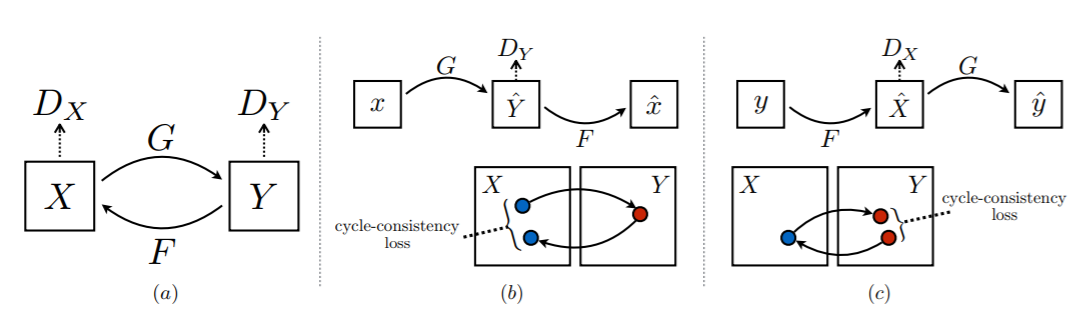
\includegraphics[width=0.95\columnwidth]{master_thesis_template/figs/cycle_gan.PNG}
    \caption[A geometric view of cycleGAN]{An illustration of mapping in cycleGAN. (a) The model contains a pair of generator discriminator networks $(F, D_Y)$ and $(G,D_X)$ where $F: X\rightarrow Y$ and $G: Y\rightarrow X$ are generator networks and $D_Y: Y\rightarrow \mathbb{R}$ and $D_X: X\rightarrow \mathbb{R}$ are corresponding discriminator networks, (b) and (c) demonstrate cycle consistency for two domains. Taken from~\cite{zhu2017unpaired}}.
    \label{fig:cycle_gan}
\end{figure}



\subsection{Unsupervised Image-to-Image Translation}
\label{subsec:unit_gan}
Unsupervised image-to-image translation (UNIT) is another GAN-based framework for the unpaired translation of images between two domain. In this thesis, our work is inspired by the UNIT framework. The UNIT (\cite{liu2017unsupervised}) is based on the assumption that two domains $X$ and $Y$ have an underlying joint probability distribution $P_{X,Y}(x,y)$ and the objective is to approximate $P_{X,Y}(x,y)$ from two marginal distributions $P_{X}(x)$ and $P_{Y}(y)$. Inferring a joint distribution from marginal distribution is an ill-posed problem. The UNIT approximates the joint probability distribution under the assumption that the two domains have a shared latent space $\mathcal{Z}$. 


Unlike cycleGAN in UNIT the two generators are expressed as encoder-decoder pairs $(E_1,G_1)$ for domain $X$, $(E_2,G_2)$ for domain $Y$ and the corresponding discriminators $D_1$ and $D_2$. For any pair of images $(x,y)$ where $x\in X$ and $y\in Y$ there exist a representation in shared latent space $z\in\mathcal{Z}$ as
\begin{equation}
    z = E_1(x) = E_2(y)
\end{equation}

and the mapping from $z\in\mathcal{Z}$ to image space is given by:
\begin{flalign}
    x = G_1(z)\\
    y=G_2(z)
\end{flalign}

The concept of shared latent space is implemented by imposing the following two conditions: (i) Weight sharing of the last layer of the encoder network and the first layer of the decoder network, (ii) cycle consistency loss. Condition (i) is a more strict condition since it also implies cycle consistency. Condition (ii) is imposed as a constraint to restrict the search space of a network and to avoid problems like the mode collapse. Figure~\ref{fig:vae-gan}
gives a geometric view of shared latent space and the UNIT network.

The VAE-GAN loss of two generators is defined as:
\begin{equation}
\begin{aligned}
V_\text{VAE-GAN} (E_1,G_1,E_2,G_2,D_1,D_2) = & V_\text{VAE} (E_1,G_1,X,Y) +  V_\text{GAN} (E_2,G_1,D_1,X,Y) \\ 
&+ V_\text{VAE} (E_2,G_2,X,Y) +  V_\text{GAN} (E_1,G_2,D_2,X,Y)
\end{aligned}
\end{equation}

The cycle consistency loss is expressed like a VAE objective function given by:
\begin{equation}
\begin{aligned}
     V_{\text{cyc}_1}(E_1,G_1,E_2,G_2) =& \lambda_1 D_{KL} (q_1(z_x|x_X) || p_{\eta}(z)) + \lambda_2 D_{KL} (q_2(z_y|x_X^{X2Y}) || p_{\eta}(z))\\
    & + \lambda_3 \mathbb{E}_{z_y\sim q_2(z_y|x_X^{X2Y})} [\log p_{G_1}(x_X|z_y)]       
\end{aligned}
\end{equation}

\begin{equation}
\begin{aligned}
    V_{\text{cyc}_2}(E_2,G_2,E_1,G_1) =& \lambda_1 D_{KL} (q_2(z_2|y_Y) || p_{\eta}(z)) + \lambda_2 D_{KL} (q_1(z_x|y_Y^{Y2X}) || p_{\eta}(z))\\
    & + \lambda_3 \mathbb{E}_{z_x\sim q_1(z_x|y_Y^{Y2X})} [\log p_{G_1}(x_X|z_x)]
\end{aligned}
\end{equation}

\begin{equation}
 V_{\text{cyc}}(E_1,G_1,E_2,G_2)  = V_{\text{cyc}_1}(E_1,G_1,E_2,G_2) + V_{\text{cyc}_2}(E_2,G_2,E_1,G_1)
\end{equation}
    
where $p_{\eta}(z)=\mathcal{N}(z|0,I)$ is a prior distribution assumed to be Gaussian,  $z_x = E_1(x) + \eta$, $z_y = E_2(y) + \eta$ and $\eta \sim p_{\eta}(z)$.
%$q_1(z_x|x_X)=\mathcal{N}(z_x|E_1(x),I)$, $q_2(z_y|x_X^{X2Y})=\mathcal{N}(z_y|E_1(x),I)$,.
The KL term ensures that the latent space distribution is close to the prior and the negative log-likelihood term is similar to the consistency term in the cycleGAN and ensures $G_1(E_2(G_2(E_1(X)))\sim X$ and $G_1(E_2(G_2(E_1(Y)))\sim Y$. 

The full optimization problem of the UNIT is expressed as:
\begin{equation}
    \begin{aligned}
        E_1^\ast, E_2^\ast, G_1^\ast, G_2^\ast, D_1^\ast, D_2^\ast =& \argmin_{E_1,G_1,E_2,G_2} \max_{D_1, D_2} V_\text{VAE-GAN} (E_1,G_1,E_2,G_2,D_1,D_2)\\
        &\qquad \qquad \qquad +  V_\text{cyc}(E_1,G_1,E_2,G_2)
    \end{aligned}
\end{equation}

\begin{figure}
    \centering
    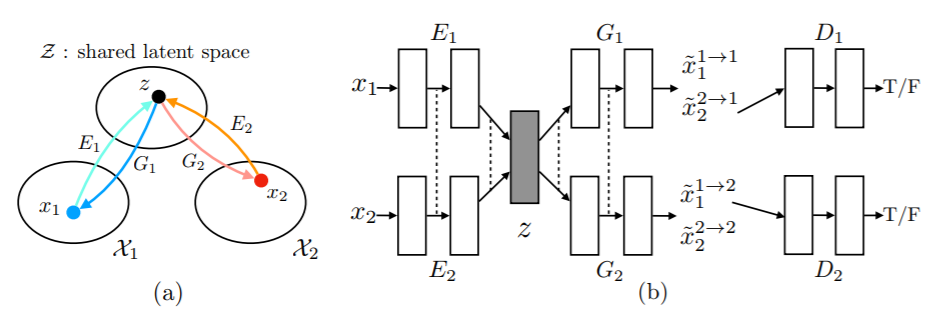
\includegraphics[width=0.95\columnwidth]{master_thesis_template/figs/unit.PNG}
    \caption[Illustration of UNIT Framework]{UNIT Network:  $(E_1,G_1)$ and $(E_2,G_2)$ are two pairs of VAEs and $D_1$ and $D_2$ are two discriminators corresponding to domain $X$ and $Y$, respectively. (a) An Illustration of shared latent space $\mathcal{Z}$. The UNIT assumes the pair $(x_1,x_2)$ can be represented by a shared latent embedding $z\in\mathcal{Z}$. (b) An example of UNIT network where dotted line illustrates weight sharing. Taken from \citet{liu2017unsupervised}.}
    \label{fig:vae-gan}
\end{figure}



\section{Deep Generative Models for Audio Signals}
\label{subsec:dganaudio}
In this section, we review recent work on deep generative models for audio signals. The recent developments in generative models in particular GANs have already achieved a lot of success for image data. However, the application to audio signals is still in the early stage. The WaveNet (\cite{oord2016wavenet}) proposed an autoregressive generative model for high-quality audio synthesis. One key drawback of this approach is that it works in the time domain and its autoregressive nature results in slow inference for audio data sampled at high frequency. 

One alternative to this approach is to use a compressed STFT representation instead of the time-domain representation of a signal. In our previous discussion, we looked at the problem of consistency and phase reconstruction associated with this approach. In a recent work \citet{engel2019gansynth} avoid the phase reconstruction and proposed a generative model that utilizes the full time-frequency representation and at inference time uses the ISTFT operation to get the time-domain waveform. To deal with the convoluted nature of phase spectra the authors transform it to an alternative representation namely the instantaneous frequency (IF). In \cite{marafiotiadversarial} the authors proposed a GAN network with an additional constraint to generate a consistent spectrogram representation in an adversarial setting. The consistency condition speeds up the learning of an iterative algorithm for phase reconstruction thus provides a better quality of the audio synthesis.

The domain adaptation of audio signals in particular of speech data offers a promising direction to improve automatic speech recognition (ASR) systems, for the development of robust speaker detection systems, privacy in end-to-end dialogue systems and many more exciting problems. \citet{hosseini2018multi} proposed a cycleGAN-based network using the spectrogram representation for cross-domain adaptation of speech signals. The approach makes use of multiple discriminators based on a frequency band to allow the generator to focus on fine-grained features.

In \citet{kaneko2017parallel} the authors proposed an architecture utilizing the cycleGAN framework for converting the voice of one speaker to another. The approach is evaluated on the VCC 2016 dataset (\cite{nakashika2016non}) of 10 speakers. In \citet{huang2018voice} the authors proposed a VAE-based architecture for voice conversion. The network jointly uses two types of spectral features in the VAE setting.
In another recent work \citet{qian2019autovc}, the authors proposed an autoencoder framework for zero-shot voice conversion. The conversion is done by incorporating speaker embedding obtained from a separate pretrained speaker classification network. The pretrained network is trained on the task of speaker identification on a large corpus of $3\,549$ speakers. Later for zero-shot voice conversion the decoder of an autoencoder network is conditioned on the embeddings obtained from the pretrained model.